\documentclass[prc,linenumbers,letterpaper,twocolumn,nofootinbib,superscriptaddress,floatfix]{revtex4-1}
  
\usepackage[utf8]{inputenc}
\usepackage{newtxtext,newtxmath}

\usepackage{amsfonts,amsmath,amssymb}
\usepackage{mathrsfs}
\usepackage{bm}

\usepackage{verbatim}
\usepackage{url}
\usepackage{graphicx}
%\usepackage{epstopdf}
\usepackage{setspace}

\usepackage[english]{babel}
\usepackage{blindtext}
\usepackage{microtype}
\usepackage[colorlinks=true,linkcolor=blue,urlcolor=blue,citecolor=blue]{hyperref}

\renewcommand{\thefootnote}{\fnsymbol{footnote}}
\def\be{\begin{eqnarray} &&} 
\def\nonu{\nonumber \\ &&} 
\def\ee{\end{eqnarray}} 
\def\nonu{\nonumber \\ &&} 

\def\lf{\left}
\def\rg{\right}

\setlength{\skip\footins}{4mm}
\setlength{\textfloatsep}{10pt plus 1pt minus 2pt}

\graphicspath{{.}{plots/}}

\date{\today}


%===============================================================================
%===============================================================================
\begin{document}

\title{Exposing Novel Quark and Gluon Effects in Nuclei}

\author{I.~C.~Clo\"et}
\affiliation{Physics Division, Argonne National Laboratory, Lemont, IL 60439, USA}

\author{R.~Dupr\'{e}}
\affiliation{Institut de Physique Nucl\'eaire, CNRS-IN2P3, Univ. Paris-Sud, Universit\'e Paris-Saclay, 91406 Orsay Cedex, France}

\author{S.~Riordan}
\email{sriordan@anl.gov (Corresponding author)}
\affiliation{Physics Division, Argonne National Laboratory, Lemont, IL 60439, USA}

\author{W.~Armstrong}
\affiliation{Physics Division, Argonne National Laboratory, Lemont, IL 60439, USA}

\author{J.~Arrington}
\affiliation{Physics Division, Argonne National Laboratory, Lemont, IL 60439, USA}

\author{W.~Cosyn}
\affiliation{Department of Physics and Astronomy, Ghent University, Proeftuinstraat 86, B9000 Ghent, Belgium}

\author{N.~Fomin}
\affiliation{University of Tennessee, Knoxville, TN 37996, USA}

\author{A.~Freese}
\affiliation{Physics Division, Argonne National Laboratory, Lemont, IL 60439, USA}

\author{S.~Fucini}
\affiliation{Perugia University and INFN, Perugia Section, via A. Pascoli snc I-06123 Perugia, Italy}

\author{D.~Gaskell}
\affiliation{Thomas Jefferson National Accelerator Facility, Newport News, VA 23606, USA}

\author{C.~E.~Keppel}
\affiliation{Thomas Jefferson National Accelerator Facility, Newport News, VA 23606, USA}

\author{G.~A.~Miller}
\affiliation{Department of Physics, University of Washington, Seattle, WA 98195-1560}

\author{E.~Pace}
\affiliation{Universit\`a di Roma ``Tor Vergata'' and INFN, Sezione di  Roma Tor Vergata, 00133 Rome, Italy}

\author{S.~Platchkov}
\affiliation{IRFU, CEA, Université Paris-Saclay, 91191 Gif-sur-Yvette, France}

\author{P.~E.~Reimer}
\affiliation{Physics Division, Argonne National Laboratory, Lemont, IL 60439, USA}

\author{S.~Scopetta}
\affiliation{Università di Perugia and INFN, Sezione di Perugia, via A. Pascoli snc I-06123 Perugia, Italy}

\author{A.~W.~Thomas}
\affiliation{ARC Centre of Excellence for Particle Physics at the Terascale and CSSM, Department of Physics,
University of Adelaide, Adelaide SA 5005, Australia}

\author{P.~Zurita}
\affiliation{Physics Department, Brookhaven National Laboratory, Upton, NY 11973, USA}

%\keywords{EMC effect; medium modification; nuclear modification; tagged scattering; deep inelastic scattering; nuclear generalized parton distributions; gluon distributions; parton distributions; short-range correlations}

\begin{abstract}
The fundamental theory of the strong interaction -- quantum chromodynamics (QCD) -- provides the foundational framework with which to describe and understand the key properties of atomic nuclei. A deep understanding of the explicit role of quarks and gluons in nuclei remains elusive however, as these effects have thus far been well-disguised by confinement effects in QCD which are encapsulated by a successful description in terms of effective hadronic degrees of freedom. The observation of the EMC effect has provided an enduring indication for explicit QCD effects in nuclei, and points to the medium modification of the bound protons and neutrons in the nuclear medium. Understanding the EMC effect is a major challenge for modern nuclear physics, and several key questions remain, such as understanding its flavor, spin, and momentum dependence. This manuscript provides a contemporary snapshot of our understanding of the role of QCD in nuclei and outlines possible pathways in experiment and theory that will help deepen our understanding of nuclei in the context of QCD.
\end{abstract}

\maketitle
\begin{spacing}{0.9}
\tableofcontents
\end{spacing}

%===============================================================================
%===============================================================================
% section I:
\section{Introduction}

The simplest picture of the partonic structure of a nucleus is one comprised of an incoherent sum of the free protons and neutrons. Deep inelastic scattering experiments strongly suggest that such a picture is at best incomplete, and therefore to gain a more detailed understanding of the quark-gluon structure of nuclei a broad program in experiment and theory must be developed.  This includes novel measurements of nuclear structure with high energy leptonic probes with inclusive, semi-inclusive and exclusive final states, Drell-Yan processes with different incident hadrons on a variety of nuclei, a rigorous development of theoretical frameworks and modeling, and careful constraint and understanding of systematic effects.

There are several key questions to be answered that are within the reach of the physics community and would broadly expand upon our present knowledge of the role of quarks and gluons in nuclei.  This includes the nature of the isovector nuclear forces and their impact on the various parton distribution functions (PDFs) of nuclei, nuclear spin-dependent PDFs, the relation between the momenta of the bound internal quarks and the hadronic constituents, and the full femtoscopic imaging of the nucleus.  Coupled with these studies is the need for a rigorous formalism and a better understanding of the systematic effects in processes such as hadronization and in the extraction of nuclear longitudinal structure functions. 

The goal of the article is to provide a status of the current experimental and theoretical understanding of the role of QCD in nuclei and to provide a road map containing a key set of questions for the next era of measurements and calculations. These new directions in experiment and theory will cover needed information for the latest nuclear parton distribution functions, programs which will study the spin and isospin-dependence of medium modification, better constrain both valence and sea distributions, and ultimately achieve a more complete tomography of the structure of nuclei. 

The structure of the article is as follows: Sec.~\ref{sec:status} provides a summary of the current status of the EMC effect; Sec.~\ref{sec:nPDFs} discusses nuclear PDFs; Sec.~\ref{sec:directions} outlines some future directions for unpolarized lepton scattering measurements including measurements of short-ranged correlations; Secs.~\ref{sec:ivemc} and \ref{sec:pemc} discuss the isovector and polarized EMC effects; Sec.~\ref{sec:DY} discusses Drell-Yan measurements; Sec.~\ref{sec:light} looks at opportunities with light nuclei such as the deuteron; Sec.~\ref{sec:lf} discusses light-front methods; Sec.~\ref{sec:tagged} studies tagged reactions; Sec.~\ref{sec:GPDs} discusses nuclear GPDs; systematic effects are studied in Sec.~\ref{sec:systematics}, and finally a summary and outlook is given in Sec.~\ref{sec:conclusion}.


% section II: Status of the EMC effect
\section{Status of the EMC effect}

One of the best tools available for studying the internal structure of nucleons is the deep inelastic
scattering (DIS) process, where a charged lepton scatters inelastically with a large four-momentum
transfer, $q^\mu$, represented by the Lorentz invariant $Q^2 = -q^\mu q_\mu \gg 1-2~\mathrm{GeV}^2$.
The process is characterized by a scaling variable Bjorken-x, $x = Q^2/2M_N \nu$, 
where $M_N$ is the mass of the target hadron and $\nu$ is the energy transferred from the lepton in the laboratory frame,
which is associated with the momentum fraction carried by a struck spin-1/2 partons in the limit of the infinite-momentum frame.
To leading order the unpolarized electromagnetic DIS cross section in the laboratory frame can be written~\cite{PhysRevD.98.030001}
\begin{equation}
    \frac{d^2 \sigma}{dx dy} = \frac{4 \pi \alpha^2}{x y Q^2} \left[ (1-y)F_2(x, Q^2) + y^2 x F_1(x, Q^2) \right]
\end{equation}
where $y = \nu/E$ where $E$ is the incident lepton energy, $\alpha$ is the fine structure constant and $F_2$
and $F_1$ are structure functions of the proton to be determined.  These structure functions can be reduced
by the Callan-Gross relation $F_2 - 2xF_1 = F_\mathrm{L} \approx 0$ for non-interacting point-like spin-1/2
particles with
\begin{equation}
    F_2(x,Q^2) = x \sum_{q} e_q^2 q(x,Q^2)
\end{equation}
where the sum $q$ is over all quark flavors,  $e_q$ is the electromagnetic chare of the quark, and the
functions $q(x,Q^2)$ are the parton distribution functions (PDFs) which are believed to be universal
and can describe other processes such as Drell-Yan scattering.  Analogous distributions exist for the case of polarized
targets.  A great success of QCD is the prediction of the logarithmic 
evolution of the PDFs with $Q^2$, the so-called DGLAP evolution.  These PDFs can in principle be measured for any bound hadronic state.

\begin{figure}[tbp]
  \centering\includegraphics[width=\columnwidth]{emc_cu_fe-crop.pdf}
  \caption{EMC effect for iron (BCDMS collaboration~\cite{Benvenuti:1987az} and SLAC E139~\cite{Gomez:1993ri})
    and copper (EMC collaboration~\cite{Ashman:1992kv}).
    Figure from Ref.~\cite{Guzey:2012yk}}
  \label{fig:emc_iron}
\end{figure}

The EMC effect~\cite{Aubert:1983xm} is the observation that the PDFs for nuclei are different than
the incoherent sum over the PDFs of the constituent nucleons and marks a clear sign of the modification
of the structure of the nucleons when bound together in a nucleus.
Since the original discovery in 1983, there has been a large
program of measurements at several laboratories, such as CERN, Fermilab, SLAC, DESY, and Jefferson Lab (JLab),
aimed at understanding the properties and probing the origin of the nuclear dependence of inelastic
structure functions (see~\cite{Geesaman:1995yd, Malace:2014uea, Hen:2016kwk} for reviews related to the EMC effect).
Measurements with high energy (of scale 100 GeV) muon beams have provided high-precision data at low to
moderate $x$ ($<0.3$), while more modest energy electron facilities (of scale 10 GeV) have provided
the highest precision at large $x$ ($>0.3$), Fig.~\ref{fig:emc_iron}.  The low-to-moderate $x$
regions show interesting shadowing and anti-shadowing behaviors, while the suppression of the
per-nucleon cross section for $0.3<x<0.7$ is the hallmark of the EMC effect.

The most comprehensive data sets with high precision at large $x$ come from SLAC E139~\cite{Gomez:1993ri} and Jlab E03-103~\cite{Seely:2009gt}. The SLAC experiment
measured the EMC effect for a wide range of nuclei, from $^4$He to Au with good precision up to
$x\approx0.8$.  One of the outcomes of E139 was an investigation of the detailed nuclear dependence of the EMC
effect. It was found that the nuclear dependence of the EMC effect at large $x$ ($x=0.6$) is consistent
with both a logarithmic $A$ dependence or a linear dependence on average nuclear density (often parametrized as an $A^{1/3}$ dependence).

The SLAC and early high energy measurements showed a number of global properties of the EMC effect:
\begin{enumerate}
 \item{The shape of the EMC effect (shadowing, anti-shadowing, and EMC regions at small, moderate, and
  large $x$ respectively) is universal and observed in all nuclei.}
 \item{The EMC effect displays little $Q^2$ dependence over the full $x$ range.}
 \item{At large $x$, the EMC effect grows with $A$, while there is little apparent $A$ dependence in the
   anti-shadowing region.}
\end{enumerate}

%%%theory
Since the first observation of the EMC effect, many theoretical models have been proposed and can be subdivided into two categories.  One includes only ``traditional'' nuclear physics effects, using convolution models with binding effects, detailed models of the nucleon momentum distribution, or pion-exchange contributions. The other category invokes more exotic explanations such as re-scaling of quark distributions in the nuclear environment, contributions of six or nine
quark bags, or modification of the internal structure of the nucleons such as ``nucleon swelling'' or suppression of point-like nucleon configurations. Several reviews give an overview of models of the EMC effect~\cite{Geesaman:1995yd, Norton:2003cb, Piller:1999wx, Hen:2013oha, Malace:2014uea}.



\subsection{EMC effect results from Jefferson Lab and the EMC-SRC correspondence}

The primary goal of Jefferson Lab E03-103 was to augment the results obtained from SLAC E139 by taking
advantage of improved target technologies to provide higher precision data for $^4$He, and the first
measurement of the EMC effect from $^3$He at large $x$.  Additional light (Be and C) and heavy (Cu and Au)
targets were also used to provide improved precision at large $x$.

Since the shape of the EMC effect is universal, the E03-103 analysis defined the ``size'' of the EMC
effect as the slope of a line fit between $0.35<x<0.7$.  This definition reduces sensitivity to
normalization uncertainties and results in higher sensitivity to the nuclear dependence.

The slope of the EMC effect for $^3$He, $^4$He, Be, and C from E03-103 plotted against scaled nuclear
density is shown in Fig.~\ref{fig:emc_jlab_hallc}.  The nuclear dependence was found to be consistent
with a simple density dependence, with the exception of $^9$Be,  which showed an anomalously larger-than-expected EMC effect given it's low average nuclear density.  However, if one considers the fact that a
beryllium nucleus can be described as two $\alpha$ clusters with an extra neutron, it then makes sense
that the EMC effect for beryllium would be more similar to $^4$He if the size of the EMC effect is
governed by the local nuclear density experienced by the quarks in the bound nucleon, rather than the
average density~\cite{Seely:2009gt, PhysRevC.82.054614}.

\begin{figure}[tbp]
  \centering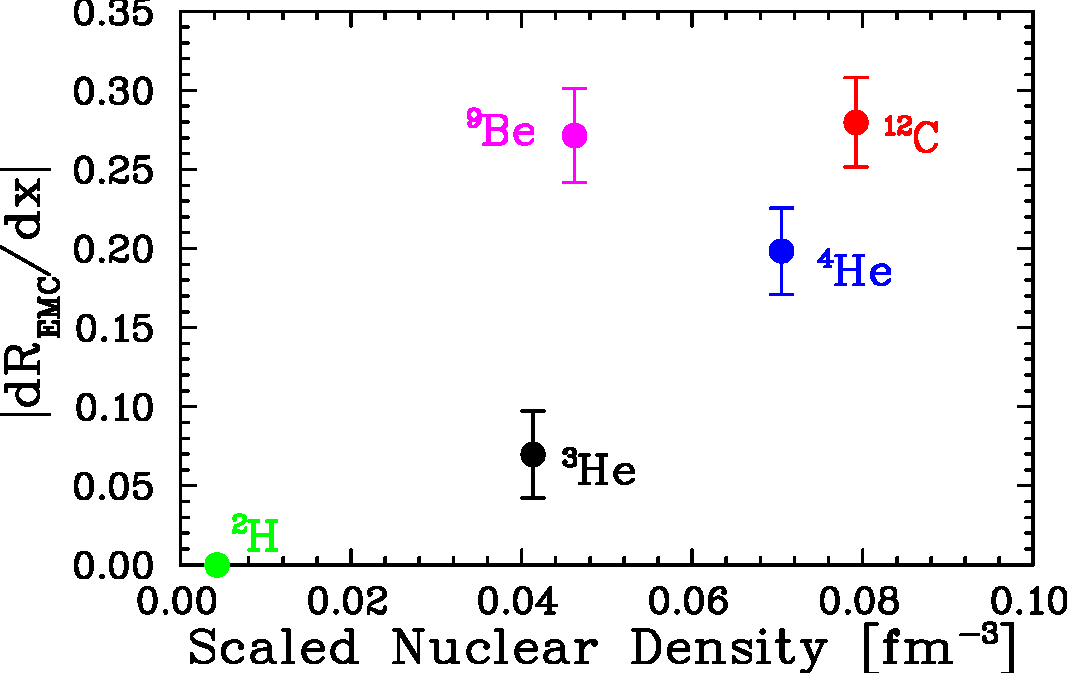
\includegraphics[width=\columnwidth]{plots/e03103_slopes.pdf}
  \caption{Size of the EMC effect (defined as $|dR/dx|$ between for $x=0.35-0.7$) vs. scaled nuclear
    density.  Figure from~\cite{Seely:2009gt}.}
  \label{fig:emc_jlab_hallc}
\end{figure}

A comparison to the $a_2=\sigma_A/\sigma_D$ ratio of
inclusive cross sections at $x>1$ (which is sensitive to the ``number of short range correlations''
found in a nucleus) a linear correlation between the two quantities was observed~\cite{Weinstein:2010rt}.
This correspondence was even more compelling when $x>1$ ratios for Be from JLab experiment E02-019 became
available and the same correlation persisted~\cite{Arrington:2012ax, Hen:2012fm}, Fig.~\ref{fig:emc_src_bff}.

\begin{figure}[tbp]
  \centering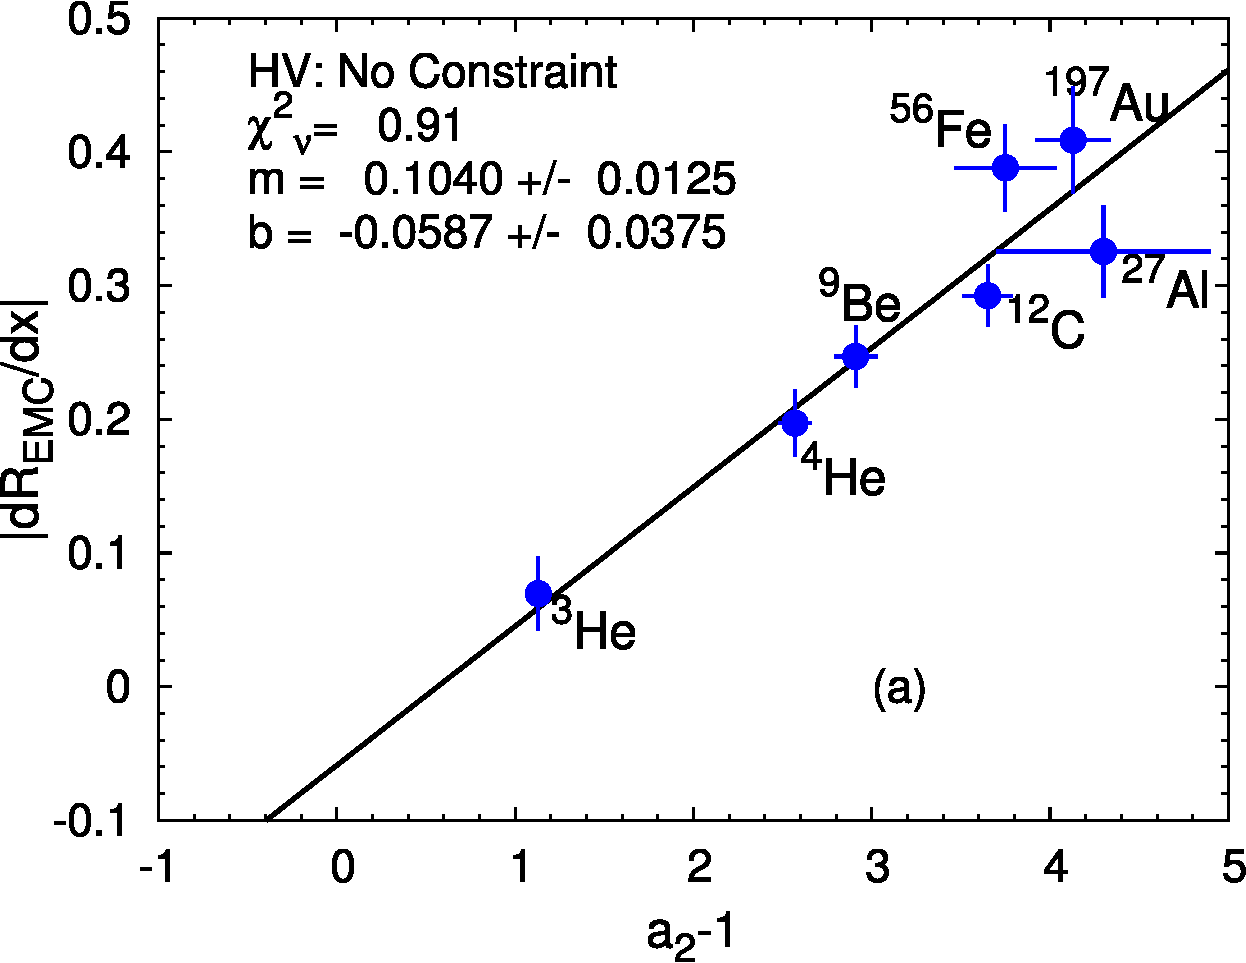
\includegraphics[width=\columnwidth]{plots/plotfit_all_norescaling_nocm_rean_final.pdf}
  \caption{Size of the EMC effect plotted vs. the SRC $a_2$ ratio. Data are from JLab and SLAC. Figure
  from Ref.~\cite{Arrington:2012ax}.}
  \label{fig:emc_src_bff}
\end{figure}

The origin of this correspondence is unclear, whether SRCs in some way cause the EMC effect, or if the two
phenomena are caused by some common underlying source.  A study was conducted to examine whether
both the EMC effect and SRCs are correlated with some other independent variable~\cite{Arrington:2012ax} such
as average nucleon separation energy, etc., with no clear common origin or factor found.

A subtlety exists in correlation studies between $x>1$ inclusive cross section ratios and the EMC effect.  The former represent the relative number of high-momentum nucleons found in an $A$ nucleus, relative to $A=2$, and not the relative number of nucleon-nucleon pairs.  This means that a causal relationsip between high-virtuality nucleons and the EMC effect can potentially represent a different scenario than one where the high-density configurations (SRC pairs) are the culprit.  Additionally, observed $NP$ dominance in SRC experiments~\cite{Subedi:2008zz} implies that for the virtuality hypotehsis, the EMC effect may differ for protons and neutrons for non-isoscalar nuclei.  Upcoming experiments at Jefferson Lab will look for signatures of such a dependence. 
\section{Quarks at $x>$1}
Quasielastic kinematics at $x>$1 probe moving nucleons, but if we increase the Q$^2$, the inelastic contribution begins to dominate, allowing us to access quark distributions. Existing JLab data have a limited range in $x$ and require the application of the of so-called "target-mass corrections" (TMCs) to extract the Q$^2\rightarrow\infty$ structure function limit.  This analysis was done for the E02-019 data, showing that the data are approaching the scaling regime~\cite{Fomin:2010ei}.  Upcoming measurements at higher energies~\cite{12gev_xgt1} can shed light on the quark structure of SRCs, where potential 6-quark configurations would result in a noticeable enhancement of the measured cross sections at $x>1$, and can be related back to the EMC region, where the enhancement is harder to determine.  Fig.~\ref{fig:quarkbags} from Ref.~\cite{Arrington:2003qt} shows the potential effect on the quark distributions in the EMC as well as the $x>1$ region.
\begin{figure}[tbp]
  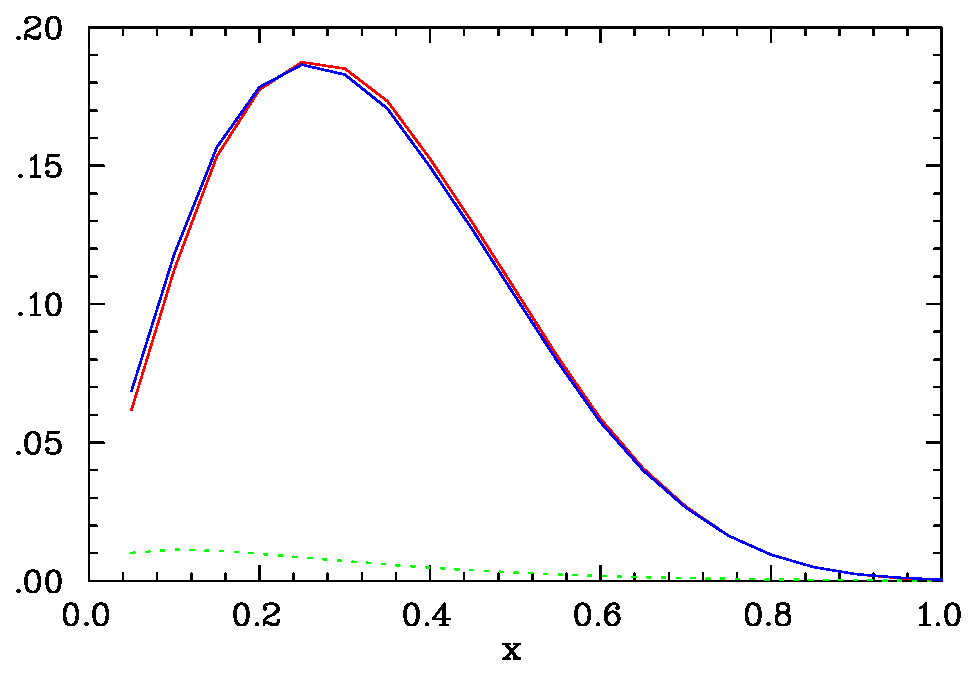
\includegraphics[width=0.45\columnwidth]{plots/qofx2_lin_5per.eps}
  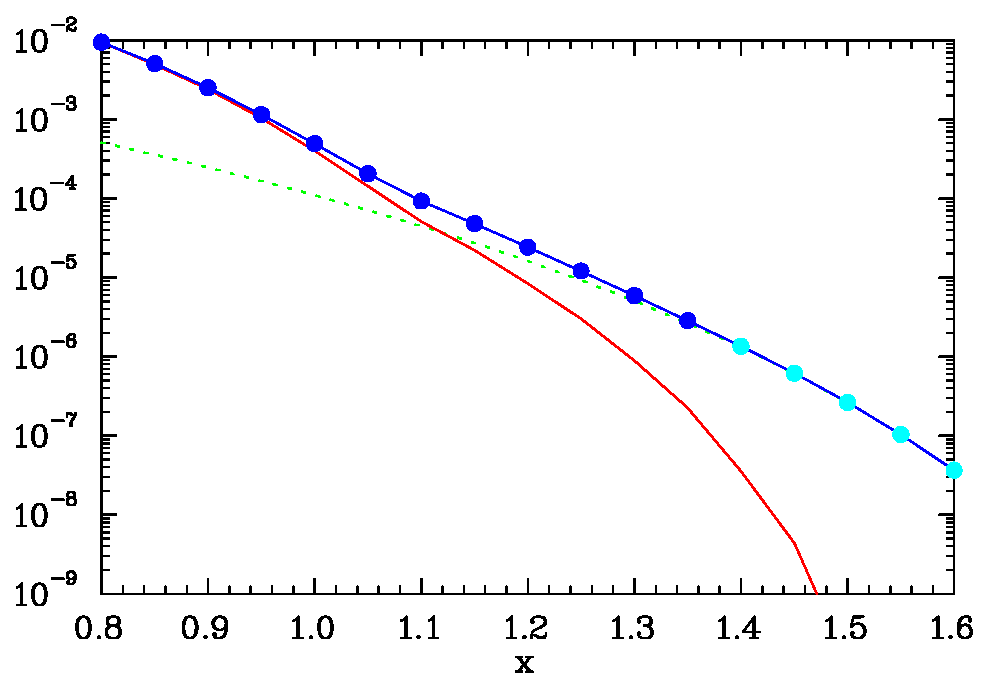
\includegraphics[width=0.45\columnwidth]{plots/qofx2_log_5per.eps}
  \caption{Quark distribution calculations for the deuteron, where the dashed line shows 2N components, the dotted line corresponds to a 5\% contribution from 6-quark bags, and the solid blue line shows the sum of the two~\cite{Mulders:1983au}. }
  \label{fig:quarkbags}
\end{figure}



% section III: Nuclear PDFs
%\documentclass[prb,11pt]{revtex4}
%\documentclass[twocolumn]{revtex4}

\section{Nuclear PDFs\label{sec:nPDFs}}
%
Nuclear parton distributions functions (nPDFs) are the first step in understanding the behavior of nuclear matter at the elementary particle level. Moreover they play a crucial role in the determination of the free proton PDFs, as nuclear targets are routinely used for separating the different partonic flavors in PDFs fits. Notwithstanding their importance, nPDFs are not as well known as the free proton case, primarily due to two factors. First, despite the phenomenal success of HERA in determining the proton structure, no electron-nucleus collider has ever existed. Second, only a few nuclei have been studied in detail and the data span a limited region of the kinematic space, to the point that the only constrained nuclear distributions are the distributions quarks in the mid-$x$ region.  For regions where data are not readily available, extrapolations for $x < 10^{-3}$ employ the fulfillment of the charge and momentum sum rules and, at mid to high-$x$, the sea quarks and gluon densities are often determined by ad-hoc assumptions during the fitting procedure, rather than from actual constraints from the data.  The parametrizations of the nuclear effects in the neutron frequently employ the assumption of isospin symmetry, which is difficult to validate given the nearly isoscalar nature of most available nuclei.

Less than about one third of the data used in nPDF fits come from heavy nuclei which complicates the possibility of truly separating the nuclear modifications for each flavor. A possible path for flavor separation would be using charged current (CC) data from DIS, which is available for iron and lead, where the cross-section depends on different combinations of the PDFs than the neutral current (NC) processes. It has been also suggested that nuclear effects might not be universal and therefore making a truly global fit of the nPDFs would not be possible. Up to now and within experimental uncertainties, NLO fits including NC and CC data have not shown visible tension. Unfortunately these fixed target experiments cover a very limited region of the kinematic space and are lacking in precision, not allowing yet for a conclusive answer.


The unexplored low-$x$ region, dominated by the gluon density, opens the possibility of finding new non-linear phenomena such saturation, and puts to test the applicability range of the linear regime. The other extreme of the kinematic space, the high-$x$ region, is of particular interest as there appears the first measured sign of nuclear effects in high energy collisions: the EMC effect. Moreover, for beyond the Standard Model searches at the LHC, rare high-$x$ gluon initiated events could be enhanced. However the nuclear gluon is difficult to access at high-$x$, and great care has to be put in its determination. Despite the lack of data, the determination of nPDFs in all the kinematic space is of crucial relevance and thus the target of several efforts. Given the fact that sea quarks and gluon densities are tied through the DGLAP evolution equations, studying processes sensitive to either sea quarks or gluons has an impact on our knowledge of nPDFs.    

\subsection{Accessing the Nuclear Gluon at High-$x$}

One of the observables in which initial state gluons can account for most of the cross-section are jets. Unfortunately the LHC measurements in jets in $p+\mathrm{Pb}$ collisions by the ATLAS collaboration~\cite{ATLAS:2014cpa} have been integrated over in the $0-90\%$ centrality bin instead of using minimum bias data, rendering the quantity difficult for comparison to collinear factorized pQCD predictions. However, the data of the di-jets measured by the CMS collaboration were published~\cite{Chatrchyan:2014hqa} and further included in the latest NLO nPDF analysis of EPPS16~\cite{Eskola:2016oht}. There it was shown that the di-jets from CMS have a non-negligible impact on the high-$x$ gluon distribution. As the EPPS16 fit comprises about $2000$ data points and allows for more flexible parametrizations, the effect of the di-jet data on constraining the gluon is less effective. %\footnote{Raphael: Is this true or just because there is little data constraining gluon distributions? I think the dilution argument is a bit spurious.}.   SPR:  I took this to just mean it has less impact. 

Nonetheless, jets remain a relevant tool to access the gluon density. In recent works~\cite{PhysRevD.95.094013, PhysRevD.97.114013} it has been shown that (di-~)jets in $e+A$ collisions at a future Electron-Ion Collider (EIC) have the potential to reduce the theoretical uncertainties by an order of magnitude at both low and high-$x$, reaching into the anti-shadowing and EMC effect regions.

A complementary way of accessing the high-$x$ gluon is using the charm quark structure function. This quantity is determined by tagging the charm in the final state and theoretically has its leading order perturbative contribution from the photon-gluon fusion process. In addition, this observable might hold the key to study if there is an intrinsic content of charm in the proton or nucleus or if heavy quarks appear only by radiation from the gluons, though fully disentangling the gluon and intrinsic charm is challenging. The studies of DIS reduced cross-section with simulated EIC data and its impact on the gluon nPDF~\cite{PhysRevD.96.114005} show that the inclusive data could reduce the uncertainty bands up to a factor of~4 at low $x$, while the charm reduced cross-section would have a dramatic effect, diminishing the uncertainties by almost an order of magnitude at high-$x$.   

\subsection{Improvements for nPDFs}

Future programs will play a key role on determining the nPDFs and it is crucial to incorporate lessons learned from prior experiments, publications, and analysis. A simple example is results from HERA where initial data were published in the form of the structure functions $F_{2}$, while in later years and after the conclusion of data taking, new publications were made of the cross-sections. The shift came from the realization that the structure functions are not a fundamental observable if considering the gluon densities and potential saturation effects. This adds uncertainty in $F_{2}$ and no reanalysis under this realization has been performed.  Similarly, assumptions are made about the form of the longitudinal structure functions $F_\mathrm{L}$ and become deeply ingrained in the results.  Corrections 
to account for the non-isoscalarity of some targets make assumptions on the flavor-dependence of the modification in nuclear data analyses and can lead to very different shapes for the EMC effect.  In this light it would be extremely beneficial for the community to publish future results which include the measured cross sections, as well as the extracted structure functions, with and without corrections or assumptions. 


% section IV: future directions inclusive
\input{texfiles/future_directions}

% section V: isovector EMC effect
\section{Isovector EMC Effects\label{sec:ivemc}}
%
One aspect of the EMC effect that has not been fully explored are isovector-dependent effects.  Such effects occur in nuclei with $N \neq Z$, e.g. many of those shown in Fig.~\ref{fig:np_ratios}, and would necessarily include degrees of freedom beyond the density, $\rho$, or nuclear mass number $A$, which has long been a method of parametrization~\cite{Malace:2014uea}.  In this situation, the nuclear $u_A$ and $d_A$ distributions can be modified separately, for example in an isovector mean field background or due to a preference in nucleon flavors in short range correlation pairing.  In a flavor separation which makes the assumption that $u_p = d_n$ and $d_p = u_n$ in the modified system, this manifests itself as an apparent charge symmetry breaking~\cite{Londergan:2009kj}, though only by the assumption that protons and neutrons retain their individual charge symmetry~\cite{Londergan:2009kj}. This assumption is not necessarily true for a bound system and can be invalid for asymmetric nuclei in the same vein as the binding energy has a symmetry energy component.  Continuing the binding energy analogy, as the symmetry energy is subleading to other bulk effects, such an isovector effect would be sub-leading to isoscalar modification effects.

The present world data have poor constraints on such an effect, in particular because many measurements of the EMC effect use symmetric or weakly asymmetric nuclei. One calculation~\cite{Cloet:2009qs,Cloet:2012td} using the Nambu-Jona-Lasinio (NJL) model and including the nuclear symmetry energy as an input, predicts deviations from the isoscalar EMC effect in the parton distribution functions on the order of several percent at large $x$.

Calculations based on SRCs predict a similar picture~\cite{Sargsian:2012sm, Arrington:2015wja}.  The observed correspondence of the short range correlation plateau with the slope of the EMC effect would indicate local densities as a driving mechanism~\cite{Weinstein:2010rt}.  Using the observation that proton-neutron pairs are found much more frequently than neutron-neutron or proton-proton pairs~\cite{Subedi:2008zz} and simple counting arguments, modification of protons and neutrons will be different in nuclei depending on the asymmetry.  In either a mean-field or SRC model, observation in the difference of quark flavors would require very high precision electromagnetic deep inelastic scattering measurements due to the suppression of the $d$ quark components weighted by the square of the electric charges. 

Weak interactions offer a novel method to probe flavor-dependent effects.  In charged-current processes, $u$ and $d$ quarks only participate in $W^-$ or $W^+$ exchange respectively. The NuTeV experiment~\cite{Zeller:2001hh} was carried out using neutrino beams at Fermilab and analyzed using the Paschos-Wolfenstein relation~\cite{Paschos:1972kj} to measure the weak mixing angle, $\sin^2\theta_\mathrm{W}$.  Due to the small neutrino cross section, heavy targets (iron) were employed which have a small neutron excess.  Charge symmetry in the bound nucleons was assumed and a significant deviation in $\sin^2\theta_\mathrm{W}$ was observed.  With the inclusion of an effect predicted by the NJL calculation noted above, much of the deviation is resolved~\cite{Cloet:2009qs,Bentz:2009yy}.  Additionally, this significantly augments neutrino scattering data which probe different flavor combinations~\cite{Schienbein:2009kk}.

%\subsection{Measuring Flavor Dependence with Parity-Violating DIS}
%
The interference between electromagnetic and neutral currents through parity-violating DIS provides a complementary process to pure electromagnetic DIS, and when used together provide a powerful method to access the flavor dependence of the EMC effect~\cite{Cloet:2012td}. In parity-violating DIS, a polarized lepton beam scattered from an unpolarized asymmetric nuclear target will form a small parity-violating cross-section between the two beam helicity states, $\sigma_{L,R}$, which at leading order is 
%
\begin{equation}
\frac{ \sigma_R - \sigma_L }{\sigma_R + \sigma_L} = -\frac{G_F\,Q^2}{4 \sqrt{2}\, \pi\, \alpha} 
\left[ Y_1(y)\,a_1(x) + Y_3(y)\,a_3(x) \right],
\label{eq:phy:apv}
\end{equation}
%
where $G_F$ is the Fermi constant, $\alpha$ the electromagnetic fine structure constant, $x = Q^2/(2M\nu)$ is the standard Bjorken-$x$ scaling variable, $M$ the mass the of nucleon, and $\nu$ the lepton energy transfer.  The $Y$ function is
%
\begin{equation}
Y_1(y) \approx 1, \qquad Y_3(y) \approx \frac{1 - (1-y)^2}{1 + (1-y)^2},
\end{equation}
%
and
%
\begin{align}
a_1(x) &= \frac{2\,\sum_q C_{1q}\, e_q\left[q(x) + \bar{q}(x)\right]}
{\sum_q\, e_q^2\left[q(x) + \bar{q}(x)\right]}, \\
a_3(x) &= \frac{2\,\sum_q C_{2q}\, e_q\left[q(x) - \bar{q}(x)\right]}
{\sum_q\, e_q^2\left[q(x) + \bar{q}(x)\right]},
\end{align}
%
where $y=\nu/E$, $E$ is the beam energy, $e_q$ is the quark electric charge couplings for flavor $q$, and $C_{1q}$ and $C_{2q}$ are the effective quark couplings dependent on the weak-mixing angle $\sin^2\theta_\mathrm{W}$~\cite{Patrignani:2016xqp}, with $C_{1u} \approx -0.19$ and $C_{1d} \approx 0.34$. The $a_1(x)$ term is dominant for fixed target, forward angle kinematics. 

The first predictions for $a_1(x)$ for $N \neq Z$ nuclei was made in Ref.~\cite{Cloet:2012td}. These calculations, which included a self-consistent isovector mean-field whose strength was fixed by the symmetry energy, found that $a_1(x)$ is particularly sensitive to flavor dependent nuclear effects such as a flavor dependent modification of the nuclear parton distribution functions. The solid line in Fig.~\ref{fig:ivemc:pvdis} presents the result $a_1(x)$ from Ref.~\cite{Cloet:2012td} for ${}^{48}$Ca, and the dashed curve is the result with no flavor dependent nuclear effects. An experiment has been proposed~\cite{emcpvdis} for the SoLID spectrometer at Jefferson Lab would be able to test the prediction from Ref.~\cite{Cloet:2012td} to better than 5-$\sigma$ with a ${}^{48}$Ca target. The projected errors for this experiment are shown in Fig.~\ref{fig:ivemc:pvdis}.

%===============================================================================
\begin{figure}[tbp]
\centering\includegraphics[width=\columnwidth]{plots/a1proj_2016.pdf}
\caption{Projected sensitivities of the quantity $a_1$ for a proposed parity-violating DIS experiment on a ${}^{48}$Ca target~\cite{emcpvdis}. The solid line is the full result from Ref.~\cite{Cloet:2012td} for $a_1$ in ${}^{48}$Ca, and the dashed line is the result when flavor-dependent nuclear effects are neglected.}
\label{fig:ivemc:pvdis}
\end{figure}
%===============================================================================







% section VI: polarized EMC effect
\input{texfiles/polarized_EMC}

% section VII: Drell-Yan and Nuclear PDFs
\input{texfiles/drell_yan}

% section VIII: Opportunities with low A nuclei
\input{texfiles/deuteron}

% section IX: Poincaré Covariant Light-Front Spectral Function and Nuclear Structure
\section{Poincar\'e Covariant Light-Front Spectral Function and Nuclear Structure\label{sec:lf}}
%
{The Poincar\'e covariant spin-dependent spectral function, proposed in \cite{PhysRevC.95.014001,Pace:2013bq,Scopetta:2014yoa,Pace:2016eiq} and based on  the light-front (LF) Hamiltonian dynamics \cite{Keister:1991sb,Dirac:1949cp},  is a useful tool for a correct relativistic treatment  of nuclear structure, suitable for the study of deep inelastic scattering (DIS) or semi-inclusive deep inelastic scattering (SIDIS) processes at high momentum transfer \cite{mar,sid1,sid2}.}
 {Indeed the Bakamjian-Thomas construction \cite{Bakamjian:1953kh} of the Poincar\'e generators
  allows one to embed the successful phenomenology for few-nucleon systems in a
Poincar\'e covariant framework.}

The LF spectral function
for a three-fermion system (as the $^3$He or a nucleon in valence approximation) depends on the  energy $\epsilon$ of the spectator subsystem  and on the LF  momentum $ \tilde{\bm \kappa}$ of the knocked out particle in the {{intrinsic reference frame of the (particle - spectator pair) cluster}}. It is built up from the overlaps of the ground eigenstate of a proper mass operator for the system \cite{PhysRevC.95.014001,Pace:2013bq,Scopetta:2014yoa,Pace:2016eiq}  and
  the tensor product of a plane wave for the particle
 times the fully interacting  state for the spectator.
 {{The use of the momentum {{${\tilde{\bm \kappa}}$}}
   allows one  to take care of macrocausality \cite{Keister:1991sb} and  to introduce
   {{a new effect of binding in the spectral function.}}}}

The LF
 spectral function
fulfills {normalization and momentum sum rule  at the same time. Integration of the spectral function on the energy
$\epsilon$
of the pair yields the LF spin-dependent momentum distribution that
can  be expressed through six scalar functions, straightforwardly obtained from the system LF wave function as integrals on the relative momentum of the spectator pair.


{{Calculations of DIS
 processes  based on a LF spectral function could indicate which is the gap with respect to the experimental data to be filled by effects of non-nucleonic degrees of freedom or by modifications of nucleon structure in nuclei.}}



% section X: 
\section{Probing the nucleus with tagged reactions} 

One of the popular methods to explain the EMC effect is that nucleons
are modified in the nuclear medium. This idea
triggered several experiments to measure the quasi-elastic 
process ($e+A \rightarrow e+p+X$). In this process, the 
elastic scattering occurs on a bound nucleon and allows the extraction of its modified 
form factor. One of the expectations from these measurements was to detect a change
in size of the bound nucleon compared to the free one. This has also motivated 
DVCS experiments, where a similar process is accessible, the so-called
incoherent nuclear DVCS ($e+A \rightarrow e+p+\gamma+X$). Results for these two 
channels are presented in Fig.~\ref{fig:QEincoh}, and show in both cases a 
significant deviation between the bound and the free nucleons. 
The difficulty with the interpretation of these measurements lies into the 
effect of final-state interactions. Indeed, the reaction products are likely
to re-interact with the remnants of the nucleus, and this affects significantly the
results. The calculation of these final state effect is complex and leads to large model 
uncertainties. 
Another problem is that in the calculation of these processes, it is important
that the initial and final-state nucleons are the same. This cannot be guaranteed
in a nucleus where one can have a off-shell nucleon in the initial state or 
have processes where a charge is exchanged and a neutron becomes a proton. For
these reasons, the debate remains open around 
the interpretation of the data on bound nucleon scatterings~\cite{Benhar:2006wy}.

\begin{figure}[tbp!]
\center
\includegraphics[width=7.6cm]{plots/ModifiedFF.png}
\includegraphics[width=8.5cm]{plots/ALU_ratioInc_x_shortscenrario.png}
\caption{Left: results of \cite{Strauch:2002wu} for the quasi-elastic form factor relative to
the plane wave impulse approximation. Right: CLAS preliminary results 
for the beam spin asymmetry in incoherent nuclear DVCS relative to the free proton DVCS.}
\label{fig:QEincoh}
\end{figure}

The solution to these problems is the tagging method, in which the nuclear fragments
are detected as illustrated in Fig.~\ref{fig:size} for the simplest case, deuterium.
In this process ($e+D \rightarrow e+p_s+X$), the high-energy electron is measured
together with the low-energy proton. The measurement of the proton in the backward 
direction ensures that it was not part of the hard interaction, thus noted with 
the $s$ subscript for spectator, and transforms the deuterium into 
an effective neutron target. First results of such a measurement
have been reported in~\cite{Baillie:2011za} with the goal to extract the structure
function of the neutron. We show in Fig.~\ref{fig:wstar} a result of this experiment
comparing the invariant mass obtained with and without the tagging method. It is 
clear that the tagging method gives a much better resolution of the structure 
present in the invariant mass distribution. Similarly to the measurement presented in 
the previous section, the main result of this experiment was however limited by the lack
of statistics. Yet, this successful measurement of a tagged process opens the way for more
experiments of the same kind in the future. 

\begin{figure}[htbp!]
\includegraphics[width=6.1cm]{plots/Wstar.png}
\caption{Neutron-electron invariant mass obtained from tagging (full points) compared 
to the invariant mass obtained
from deuterium data (hollow points)~\cite{Baillie:2011za}.}
\label{fig:wstar}
\end{figure}

The nuclear tagging is the extension of the deuterium tagging to heavier nuclei, which
consists in measuring the reaction ($e+A \rightarrow e+(A-1)_s+X$), with
$(A-1)_s$ the spectator remnant of the nuclear target. This measurement is very 
interesting as it gives a direct information on which nucleon was hit by the 
deeply inelastic electron scattering in the nucleus. Also, by selecting 
low momentum backward emission of the $(A-1)_s$, we can suppress the 
final state interactions that are often a problem in such nuclear reactions. 
Detailed studies~\cite{CiofidegliAtti:2003pb,Alvioli:2006jd} have indeed shown 
that the final state interactions effects are minimized when the nuclear recoil
is detected in a backward angle relative to 
the virtual photon direction and maximized in perpendicular kinematics.
The detection of such recoil nuclei is however extremely challenging.

Tagging recoiling remnants has another interest in the quest to understand nuclear structure.
The kinematics of the nuclear remnants contain information on the
initial state of the nucleons in the nucleus. By performing at the same time the 
tagging and a deeply inelastic scattering, we probe simultaneously the nucleon and the 
quark structure of the nucleus. Tagging is therefore a unique tool to relate the EMC
effect to more classical nuclear effects and see if there is any correlation between
them. The more natural variable to use for these studies is the nucleon virtuality.
It can be calculated~\cite{CiofidegliAtti:2007ork} in the impulse 
approximation, where the nucleon momentum is exactly $\mathbf{p} = -\mathbf{P}_{A-1}$, 
giving:
\begin{equation}
v(|\mathbf{p}|, E) = \left (M_A - \sqrt{(M_A - m_N + E)^2 + \mathbf{p}^2} \right )^2 
                   - \mathbf{p}^2 - m_N^2,
\end{equation} 
where $E$ is the removal energy, $M_A$ the mass of the target nucleus
and $m_N$ the mass of the nucleon. The nucleon virtuality is a key 
observable to understand the nuclear quark and gluon structure,
as there are radically different predictions for its impact on the partonic structure.
Indeed, the descriptions of the EMC effect based on nucleon dynamic 
predict a strong correlation between virtuality and nucleon modification,
while the ones involving other hadronic degrees of 
freedom or mean field effects do not. 

Nuclear tagging measurements have never been performed in the past
on nuclei with $A>2$ due to detector limitations. Indeed, the radial TPC used 
for the experiments described above~\cite{Baillie:2011za}
is unable to differentiate isotopes and thus ensure the identification of 
nuclear remnants. There are plans at Jefferson Lab to remediate this issue
with the construction of a new detector to perform nuclear tagging measurements 
for the first time~\cite{Armstrong:2017zqr,Armstrong:2017zcm}.



% section XI: GPDs of Nuclei
\input{texfiles/gpds}

% section XII: Systematics
\section{Systematics\label{sec:systematics}}


\subsection{Hadronization and Final State Effects}

The formation of hadrons and the propagation of quarks in a nuclear medium is important for interpreting the final states of reactions in semi-inclusive DIS and Drell-Yan processes as well as critical for interpreting gluon distributions.  An important open question are the relative sizes of the interactions between asymptotic quark propagation and interactions after hadronization.  As final states can reveal important information regarding the kinematics (such as Bjorken $x$) and flavor in a given interaction, improving the quality studies and models will simultaneously improve the extraction of modification data.  Studies have taken place at a variety of facilities, e.g. Fermilab~\cite{PhysRevC.75.035206}, JLab~\cite{PhysRevLett.99.242502, ELFASSI2012326}, and HERMES~\cite{Airapetian2011} as well as a future program with CLAS12 at JLab to study this in a broad set of channels~\cite{quarkformprop}.

Determination of the gluon distributions are also contaminated by final state interactions. nPDFs have been including routinely particle production in $d+\mathrm{Au}$ collisions into the fits, an observable that is very sensitive to both the initial state and hadronization of the gluon. The fragmentation functions for pion production have been best determined from $e^+e^-$ data, though the fragmentation of gluons have a sizable theoretical uncertainty. Data from the LHC at $7$~TeV can not be well described by a global fit unless a significant cut in $p_{T}$ is applied to the data, leaving out a relevant portion of the covered $d+\mathrm{Au}$ region.  With the present data, this constitutes a sizable source of uncertainty for the extraction of the nPDFs and conclusions from incorporating particle production data from hadron colliders into the fits must be drawn carefully.

\subsection{Free Nucleon Parton Distributions}

While the free proton parton distributions have been studied extensively and with great precision, there still remain important measurements to be done to constrain the two leading-flavor parton distributions, in particular in the ratio of $d/u$ limit as $x \rightarrow 1$.  As these represent the basis of comparison for any nuclear modification effect, it is critical to have high quality data available, especially as one considers doing flavor decompositions of nuclei.  There are several programs which intend to improve the fixed-target lepton scattering data, such as using the ratio of ${}^{3}$H and ${}^{3}$He cross section~\cite{mar}, tagged spectator with deuterium~\cite{bonus12}, and parity-violating deep inelastic scattering on the proton~\cite{solid_pvdis}.  In addition, recent analyses of $W$ and $Z$ production in $p\bar{p}$ collisions from the CDF and D\O\ collaborations~\cite{D0:2014kma,Abazov:2013dsa,Acosta:2005ud,Aaltonen:2009ta,Aaltonen:2010zza,Abazov:2007jy} have also provided new constraints at large $x$ and have been incorporated into a recent global PDF analysis~\cite{Accardi:2016qay}.



% section XIII: conclusion
\section{Summary and Key Issues}

The area of medium modification in nuclei has been a rich field for several decades and here we have provided a survey of the outstanding issues to be addressed.  To continue to advance this field in a coherent manner, a world-wide effort is required on a broad number of topics.  We identify some of the most urgent questions along with their programs.

\begin{itemize}
    \item{What is the isovector nature of the EMC effect?  This requires a set of high-precision experiments across nuclei of traditional inclusive cross section ratios, electroweak measurements which are sensitive to unique quark flavor combinations, and Drell-Yan experiments.  These would be complemented by exclusive isotope tagging experiments.}
    \item{What is the spin dependence of the EMC effect?  There is no experimental information available and any such measurement would break into new ground and would provide new information on potential mechanisms.}
    \item{What is the momentum-dependence of the EMC effect?  This can be addressed through tagged scattering measurements which can separate local density and mean field mechanisms.}
    \item{What is the image of the full nucleus in terms of both quarks and gluons?  The study of generalized parton distributions through deeply virtual Compton scattering and deeply virtual meson production as well as at existing and future colliders are critical in producing a unified femtoscopic map of the nucleus.}
\end{itemize}

\section{Acknowledgements}

The authors are grateful to the ECT* in Trento, Italy for the support and for hosting the workshop ``Exposing Novel Quark and Gluon Effects in Nuclei'' in 2018 which made this work possible.  Argonne National Laboratory's work was supported by the U.S. Department of Energy, Office of Science, Office of Nuclear Physics, under contract DE-AC02-06CH11357.  



%===============================================================================
%===============================================================================
\begin{acknowledgments}
The authors are grateful to the ECT* in Trento, Italy, for the hosting the workshop ``Exposing Novel Quark and Gluon Effects in Nuclei'' in April 2018 which made this work possible.  
%
The U.S. Department of Energy, Office of Science, Office of Nuclear Physics supported contributions from Argonne National Laboratory under contract DE-AC02-06CH11357. The contributions from the University of Tennesee, Knoxville, were supported by grant DE-SC0013615; contributions from the University of Washington were supported under Award Number DE-FG02-97ER-41014; and contributions from the University of Adelaide were supported by the Australian Research Council through the ARC Centre of Excellence for Particle Physics at the Terascale (CE110001104) and Discovery Project DP15110310.
\end{acknowledgments}


\bibliography{fullbib}

\end{document}



